%------------------------------------------------------------------------------------
%	CHAPTER 2
%------------------------------------------------------------------------------------
\chapterimage{headerCap.png}
\chapter{Falando com Ubuntu}

\begin{remark}
O computador não é mais apenas um dispositivo, é uma extensão da sua mente e uma porta de outra para a mente dos outros. (Mark Shuttleworth) 
\end{remark}

\section{Coisas Ubuntu}\index{Falando com Ubuntu}
Acho muito engraçado como existe um caso de paixão ou puro ódio em relação a Ubuntu. Não sei se é inveja por ser a distribuição mais utilizada, ou chateação pois é muito fácil de usar, ou simples paranoia mesmo. Alguns defensores radicais do software livre pregam que Ubuntu não é 100\% Software Aberto, pergunto, e daí? Vamos imaginar que a \textbf{NVidia} produziu um drive para sua placa e a empresa simplesmente resolveu não divulgar os fontes, qual o problema disso? Quero saber é: A placa que paguei bons quantos dólares (porque não foi em reais) vai funcionar com aquele super jogo, ou devo (como bom usuário do Software Livre) exigir que no meu computador só entre software aonde posso ver os fontes senão estarei ``defraudando'' alguma organização.

Outra alegação em ser tudo aberto é porque senão a \textbf{Canonical} pode enviar informações do meu computador sobre o que estou fazendo. Falando sério, acredita realmente que Google, Microsoft, Oracle, Canonical ou qualquer outra empresa está interessada no que está fazendo? Essas empresas estão interessados é no que o coletivo está fazendo, pois precisam desses dados como forma de prospectar novos negócios, é uma simples pesquisa no qual somos todos participantes ativos. Não gosta disso? Então recomendo que desligue sua Internet, tire a bateria de seu telefone, puxe o cabo da tomada da televisão, tire as pilhas do rádio, quebre seu cartão de crédito e não esqueça de levar um colchão (de palha) para a caverna que pretende morar a partir de hoje.

Caso contrário, siga os seguintes passos: \vspace{-1em}
\begin{enumerate}[noitemsep]
 \item Abrir o aplicativo \textbf{Programas e atualizações}
 \item Na aba \textbf{Drives Adicionais}, ativar (caso exista) os drivers proprietários (NVIDIA, ATI, Broadcom)
 \item Na aba \textbf{Outros Programas}, ativar o repositório ``Parceiros da Canonical'' para ter acesso a alguns aplicativos extras.
\end{enumerate}

Quando, ainda na versão da interface gráfica Unity, surgiu a barra lateral e muita gente não gostou. Só que esta barra contém os aplicativos que estão abertos e ao posicionar o mouse sobre eles e usar o scroll (a rodinha do meio) é trazido para a tela da frente, ou seja, tornou muito mais fácil e rápido acessar qualquer aplicativo. A barra foi tão importante que no retorno do Gnome decidiram criar uma versão desta.

Outro xingamento em relação a interface gráfica Unity foi que muitos usuários de Linux nasceram acostumados com o KDE ou o Gnome, e esse último era o padrão do Ubuntu até ser substituído pela Unity. Como nasci para este mundo na 14.04 não sei se o Gnome era melhor (pois quando usava achava sempre mais bonito o KDE do Kurumin), só que o Unity além de muito fácil em configurar, junto com o Compiz permitia que personalizasse a área de trabalho do jeito que gosto. Com a volta do Gnome simplesmente me adaptei sem me importar muito.

Acho que o real problema das pessoas é que não gostam de \textbf{mudanças}. Estamos ali naquela tranquilidade em um ambiente que conhecemos e de repente, acontece. Alguém vem com uma ideia doida e tudo muda, acho que mudança faz parte do mundo. Desde que me conheço por gente, se não me adaptasse hoje estaria programando em um terminal com PL1 ou Algol. Uma das características principais do ser humano e adaptação, porém primeiro existe a reclamação. 

Não sou e nem pretendo ser vítima disso que as pessoas pregam sobre Ubuntu, escolhi porque achei a distribuição mais fácil e mais agradável de lidar e até o momento não me arrependo da decisão e no dia que mudar será porque descobri algo melhor e mais fácil de utilizar.

\subsection{Curiosidade das Versões}\index{Conceitos Introdutórios}
Por ano são lançadas 2 versões do Ubuntu, por exemplo em 2014 foram lançadas as versões 14.04 e 14.10. O primeiro número corresponde ao ano da versão e o número adjacente ao seu mês de lançamento. Então, 14.04 foi lançada no mês de abril enquanto que a 14.10 lançada no mês de outubro no ano de 2014. Outro detalhe é que a primeira normalmente traz mudanças mais profundas enquanto que a segunda fica a cargo de um pacote completo de correções (como aqueles famosos \textit{Service Packs} lançados pela Microsoft) ou seja, se quiser muita estabilidade opte sempre pela segunda ou versões LTS.

Uma versão LTS significa que possui um longo tempo de suporte (\textit{Long Term Support}) e atualmente significa que a versão terá suporte oficial da Canonical por 5 anos. As outras são subtituladas Regulares (\textit{Regular}) que são como laboratórios de testes para as versões LTS, seu suporte é de 2 anos e utilizam os pacotes mais recentes.

Eis uma lista com todas as versões lançadas até este livro:
\begin{center}
 \begin{longtable}[h!]{l|l|l}
  \textbf{Versão} & \textbf{Code Name – Animal} & \textbf{Kernel} \\
  \hline
  4.10 & Warty Warthog (O porco-africano verruguento) & 2.6.8 \\
  5.04 & Hoary Hedgehog (O ouriço grisalho) & 2.6.10 \\
  5.10 & Breezy Badger (O texugo fresco) & 2.6.12 \\
  6.06 LTS & Dapper Drake (O pato doméstico estiloso) & 2.6.15 \\
  6.10 & Edgy Eft (A salamandra hi-tec) & 2.6.17 \\
  7.04 & Faisty Fawn (O cervo jovem bravo) & 2.6.20 \\
  7.10 & Gutsy Gibbon (O gibão1 corajoso) & 2.6.22 \\
  8.04 LTS & Hardy Heron (A garça durona) & 2.6.24 \\
  8.10 & Intrepid Ibex (O bode intrépido) & 2.6.27 \\
  9.04 & Jaunty Jackalope2 (A coelho antílope elegante) & 2.6.28 \\
  9.10 & Karmic Koala (O koala kármico) & 2.6.31 \\
  10.04 LTS & Lucid Lynx (O lince lúcido) & 2.6.32 \\
  10.10 & Maverick Meerkat (O suricate vagabundo) & 2.6.35 \\
  11.04 & Natty Narwhal (O narval inteligente) & 2.6.38 \\
  11.10 & Oneiric Ocelot (A jaguatirica onírica) & 3.0 \\
  12.04 LTS & Precise Pangolin (O pangolim preciso) & 3.2 \\
  12.10 & Quantal Quetzal (o quetzal quântico) & 3.5 \\
  13.04 & Raring Ringtail (O bassarisco ávido) & 3.8 \\
  13.10 & Saucy Salamander (A salamandra atrevida) & 3.11 \\
  14.04 LTS & Trusty Tair (A cabra selvagem fiel) & 3.13 \\
  14.10 & Utopic Unicorn (O unicornio utópico) & 3.16 \\
  15.04 & Vivid Vervet (O macaco vívido) & 3.19 \\
  15.10 & Wily Werewolf (O lobisomem astuto) & 4.1 \\
  16.04 LTS & Xenial Xerus (O xerus hospitalário) & 4.4 \\
  16.10 & Yakkety Yak (O iaque falador) & 4.8 \\
  17.04 & Zetty Zapus (O zapus enérgico) & 4.10 \\
  17.10 & Artful Aardvark (O porco-formigueiro astuto) & 4.13 \\
  18.04 LTS & Bionic Beaver (O castor biônico) & 4.15 \\
  18.10 & Cosmic Cuttlefish (O choco côsmico) & 4.18 \\
  19.04 & Disco Dingo (O dingo dançante) & 5.0 \\
  19.10 & Eoan Ermine (O eoan arminho) & 5.3 \\
  20.04 LTS & Focal Fossa (A fossa focal) & 5.4
 \end{longtable}
\end{center}\vspace{-3em}

Os ``apelidos'' dados para cada versão é a formação das palavras \textbf{adjetivo + animal}. E esse adjetivo não é uma palavra qualquer, possui a mesma letra inicial do animal em questão, e que a partir da versão 6.06 possui uma sequencia alfabética.
\\[3mm]
\begin{dica}[Não precisa instalar o Ubuntu para usá-lo]
	Nem ao menos colocar um DVD (ou CD) Live, basta acessar o seguinte endereço \url{http://www.ubuntu.com/tour/en/} para entrar em um simulador. Experimente pois é totalmente indolor. \url{http://old-releases.ubuntu.com/releases/} este site é para todo tipo de saudosista que deseja encontrar uma versão antiga do Ubuntu.
\end{dica}

\subsection{Como atualizar a versão do sistema?}\index{Conceitos Introdutórios}
Se já possui o Ubuntu instalado a atualização é realizada através da confirmação do desejo de instalar uma nova versão. Para que a janela de escolha possa ser mostrada, abra o aplicativo “Programas e Atualizações” e na aba “Atualizações”, verifique se a opção “Notificar-me de uma nova versão do Ubuntu” está selecionada com a escolha a qualquer nova versão.
\begin{figure}[H]
 \centering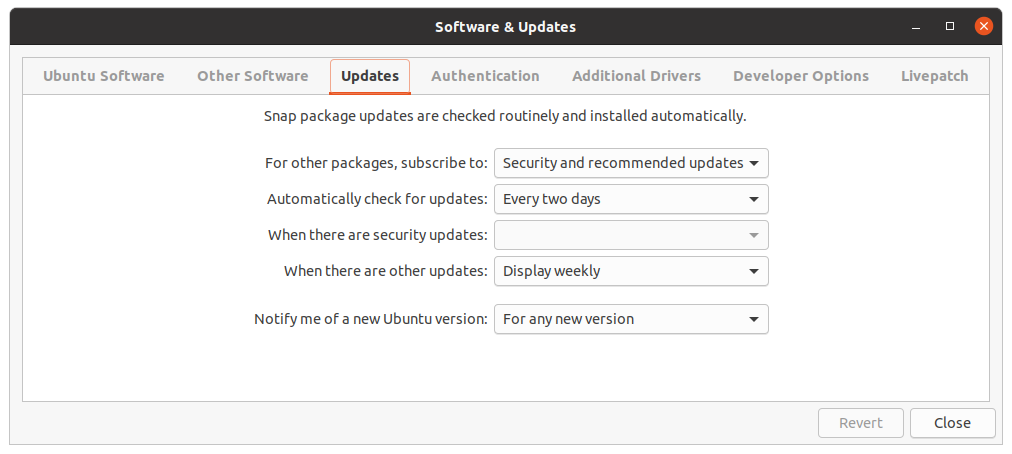
\includegraphics[scale=0.4]{cap02/atualizar.png}
 \caption{Verificar esta opção}
 \end{figure}

Se desejar que a atualização seja realizada agora, entrar no terminal e usar os seguintes comandos: \\
{\ttfamily\$ sudo apt update \&\& sudo apt dist-upgrade \\
\$ sudo do-release-upgrade}

\section{Termos usados pelos usuários}\index{Falando com Ubuntu}
Caso venha a participar de listas de discussão ou de conversas sobre o Linux é bem provável que ouça uns termos que não ouviria em discussões sobre o Windows. E esses termos não se restringe apenas a Kernel ou Distros, vai muito além disso, vejamos os mais comuns:
\begin{itemize} \vspace{-1em}
   \item \textbf{Boot Loader} – refere-se ao programa de inicialização, é aquele programa que define qual sistema operacional será chamado. Por exemplo: GRUB ou ISOLINUX.
   \item \textbf{Serviços ou Processos} – são os aplicativos que estão rodando em background no computador neste exato momento.
   \item \textbf{File System} – a forma como são organizados e armazenados seus arquivos no sistema operacional, isso é definido durante o processo de formatação. Por exemplo: ext3, ext4, FAT, XFS e NTFS.
   \item \textbf{X Window} – refere-se a toda interface gráfica, formada por: Ambiente Desktop, Gerenciador de Janelas e X11 (sistema X Window).
   \item \textbf{Ambiente Desktop} – refere-se ao ambiente gráfico que visualizamos que pode ser, GNOME, KDE, Xfce, Fluxbox e Unity.
   \item \textbf{Linha de Comando} – é a interface para digitar os comandos (a janela de terminal).
   \item \textbf{Shell} – é o interpretador de comandos, sua função é de interpretar o comando dado no terminal e diz ao sistema operacional o que fazer.
\end{itemize}
Existem também alguns comandos que todo administrador do sistema conhece e muitas vezes são utilizados nas lista de discussão para a resolução de um determinado problema.

Mostrar todas as mensagens do Kernel, é útil para resolução de problemas de inicialização do sistema ou algum erro que pode estar acontecendo recorrentemente: \\
{\ttfamily\$ dmesg}

Observar detalhes da CPU: \\
{\ttfamily\$ cat /proc/cpuinfo}

Observar detalhes da memória: \\
{\ttfamily\$ cat /proc/meminfo}

Verificar quando ocorreram as últimas inicializações ocorridas no sistema: \\
{\ttfamily\$ last reboot}

Descobrir se existe alguém ``pendurado'' no nosso computador: \\
{\ttfamily\$ w}

\section{Reiniciar o ambiente gráfico}\index{Falando com Ubuntu}
Fiquei pensando que meu problema com o Windows poderia ter sido resolvido com algo bem simples – Reiniciar as propriedades gráficas. Por exemplo, acabamos de instalar um drive para uma placa gráfica e arrebentamos completamente com a interface gráfica. E o que desejo propor é muito simples: Sem nenhum ponto de restauração desejo aplicar um RESET nas propriedades gráficas e voltá-las ao padrão do qual estavam quando instalei o sistema. Tenho diversos aplicativos instalados, não quero perdê-los e não tenho nenhum ponto de restauração.

E esse é o grande problema do Windows, muitas coisas são tão voltadas ao iniciante que o sistema esquece que existem usuários mais avançados para corrompê-lo. Outra problema é ser administrador de um curso de informática, são vários computadores e ao finalizar uma turma cada computador apresenta uma cara diferente (além de outras coisas). Existem soluções Windows para isso? Claro que sim, vamos a algumas: \vspace{-1em}
\begin{itemize}[noitemsep]
 \item Criar um ponto de restauração antes da aula, e usá-lo depois. Problema: Perderemos qualquer coisa que o professor tenha instalado. 
 \item Criar uma imagem do sistema e restaurá-lo em seguida. Problema: O mesmo anterior. 
 \item Não permitir que o aluno altere qualquer coisa no sistema operacional. Problema: E como o aluno vai instalar os aplicativos que o professor deseja? Vai ter que acabar permitindo que sejam instalados pelo aluno.
 \item Ter máquinas com tudo previamente instalado. Problema: Adeus aula prática de instalação e o aluno que se vire em casa para instalar tudo.
\end{itemize}

Ou seja, em qualquer dessas soluções acabamos esbarrando em problemas. Isso porque nem citei a solução de aplicativos que fazem esse controle e que envolvem custos. Quero permitir (assim como ter) liberdade de poder mudar o sistema da forma como quiser e depois, se algo der errado, magicamente, dar um comando RESET e tudo voltar a normalidade. Para reiniciar o ambiente gráfico GNome necessitamos realizar os seguintes passos no terminal.

Acessar o diretório: \\
{\ttfamily\$ cd /etc/init.d}

Para reiniciar a interface gráfica: \\
{\ttfamily\$ sudo service gdm restart}

Para interromper a interface gráfica: \\
{\ttfamily\$ sudo service gdm stop}

Para iniciar a interface gráfica: \\
{\ttfamily\$ sudo service gdm start}
\\[3mm]
\begin{dica}[Não se desespere] Utilize esses comandos quando a coisa estiver realmente feia, lembre-se que é sempre ideal ter uma cópia de segurança de todos seus arquivos particulares. 

Outra dica, muitas das configurações particulares dos aplicativos ficam na pasta: $\sim$/.config então, em muitos dos casos basta eliminar a configuração particular de um determinado aplicativo em questão que possa estar apresentando problemas.
\end{dica}

Sua interface está lenta ou estranha? Não é necessário sair da sessão ou reiniciar tudo, basta pressionar \textbf{ALT + F2} e digitar o comando ``r''.

\section{Existe vida além do Ubuntu}\index{Falando com Ubuntu}
Ubuntu não é a única distribuição filha da Debian e derivam várias outras distribuições, entre as mais conhecidas estão: \vspace{-1em}
\begin{itemize}
 \item \textbf{Ubuntu Studio} – Provavelmente se não usasse Ubuntu seria esta distro que usaria, vem com muitos aplicativos instalados para transformar o computador em uma central de edição de Música, Imagem e Vídeo.
 \item \textbf{Xubuntu} – Com base em Xfce que, segundo seus criadores, busca ser um sistema elegante e muito fácil de usar.
 \item \textbf{Kubuntu} – Com base em KDE. É uma alternativa ao uso do Gnome e Unity fortemente presentes e por muito pouco não foi minha distribuição escolhida pois gostava muito do visual da distribuição Mandriva (da Conectiva).
 \item \textbf{Edubuntu} – Totalmente focada para ser a distribuição ideal para escolas e estudantes em geral.
 \item \textbf{Linux Mint} – É a grande concorrente, e busca a facilidade de uso através de um ambiente gráfico visualmente explorado.
 \item \textbf{Knoppix} – é uma Live CD também baseado em KDE.
 \item \textbf{Kanotix} – é a que mais se parece com a Avó (Debian) sendo também uma Live CD.
 \item \textbf{Damm Small Linux} – Este é a pequenininha da família (possui apenas 50 Mb) é outra Live CD baseado na Knoppix.
\end{itemize}

As quatro primeiras distros são basicamente uma cópia da Ubuntu destinadas as suas particularidades. No Brasil, o Governo Federal lançou a \textbf{Linux Educacional}\footnote{Em \url{https://linuxeducacional.c3sl.ufpr.br/}} também com base na Ubuntu (pode-se dizer que é uma Edubuntu Brasileiro) que nasceu no Centro de Experimentação em Tecnologia Educacional (CETE) do Ministério da Educação (MEC) e atualmente (na versão 6.1) está a cargo da Universidade Federal do Paraná. E foi exatamente esta distribuição que me fez voltar a utilizar o Linux.

\section{Janela do Terminal}\index{Falando com Ubuntu}
A primeira vez que tentei utilizar Linux na vida foi quando comprei um livro, ``Servidor Internet com Linux'' de Kevin Reichard, vinha com um CD com o \textbf{Slackware OS - Versão 2.2}. Quando um colega que entendia muito do Linux conseguiu instalar no meu computador juro que me senti como se tivesse adquirido um daqueles extremamente antigos, cadê a janela gráfica que o Windows 3.11 possuía e que facilitava muito meu trabalho? Como iria instalar meus aplicativos? O que iria fazer com um sistema operacional que tinha uma tela estranha para mim, não tinha a menor noção dos comandos e a linguagem C como pano de fundo\footnote{Para entender meu drama, era um programador oriundo do Pascal}.
\begin{figure}[H]
 \centering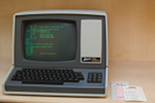
\includegraphics[scale=4.5]{cap02/computadorAntigo.png}
 \caption{Computador antigo da minha época}
\end{figure}

Minha segunda tentativa foi durante o planejamento do meu livro de PHP, tinha uma pilha de CDs de distros, tinha adquirido naquelas revista que se encontrava aos quilos nas bancas (outra metade dos meus CDs eram Demos de jogos – Sim, houve época que nos divertíamos com uma ou duas fases de um jogo e isso durava horas). Como o PHP, Apache e MySQL eram totalmente livres nada mais justo seria que também usasse um sistema livre para o livro, só que queria que a instalação fosse fácil para meu leitor (afinal não estaria ao seu lado para instalar o ambiente). Funcionava assim, pegava um CD, instalava a distro, tentava colocar o Apache e um editor de modo simples (em muitas o MySQL já vinha instalado por padrão), não dava muito certo (ou era muito complicado) e então mudava de distro (e de CD) o que significava ter que formatar novamente o computador. Resultado que meus dois livros de PHP são escritos para o Windows.

Vou ser bem franco, achava o Linux um Sistema Operacional para os outros. Ainda tentei usar sem muito sucesso me adaptar a Kurumin (uma LiveCD brasileiro) e a Mandriva, mas em momento nenhum via isso como substituto ao Windows, eram apenas para pessoas que adoravam perder muito tempo em fazer algo que resolvia com alguns cliques.

Durante muito tempo achei que nunca usaria esse sistema, até um dia que meu filho meu deu seu Netbook e, não sei porque, resolvi instalar o \textbf{Linux Educacional}, finalmente vi que tinham domesticado o Pinguim e que poderia ser usado para alguma coisa boa. Usei esse computador na faculdade e em nenhum momento me arrependi.

Minha mudança definitiva aconteceu com todos os problemas que citei no começo deste livro, resolvi usar o Linux mais uma vez e de vez. Uma as recomendações que recebi foi: ``Instale o sistema sem a parte gráfica que aprenderá muito mais'', devo confessar que foi a coisa mais IDIOTA que ouvi nos meus 25 anos de informática. Isso soou como alguém dizendo: ``Jogue fora seu computador e use novamente seu TK-83C ou que tal trocar o LibreOffice pelo WordStar ou RedatorPC''.

Quero meu computador para editorar esse livro, fazer meu trabalho da faculdade, programar com um belo editor colorido, baixar a interface do Arduíno, usar aplicativos que comumente uso no meu trabalho, assistir um vídeo, ouvir uma boa música e por aí vai e isso não tem nada a ver com \textbf{ps aux | grep [nome]} e boa sorte para quem sabe o que isso faz.
\\[3mm]
\begin{dica}[Consoles do Linux] Quer ter a experiência de ficar puramente em modo terminal? Então pressione as teclas \textbf{Ctrl + Alt + F2} (existem 6 consoles do F1 a F6). Para retornar ao modo gráfico pressione as teclas \textbf{Ctrl + Alt + F1}.
\end{dica}

No que puder evitar de usar o terminal, evitarei. Não espere encontrar aqui referência aos comandos \textbf{tail} ou \textbf{cd}, o que é a pasta \textbf{/etc} ou \textbf{/opt} ou qualquer coisas dessas. Tentarei e irei simplificar tudo ao máximo, algumas vezes teremos que botar um pouco a mão no terminal mas nada que consiga assustá-lo muito e talvez consigamos aprender a usá-lo sem muitos problemas. Garanto que atualmente a coisa mais interessante a se fazer em uma janela do terminal é digitar o seguinte comando: \\
{\ttfamily\$ apt moo}

Para aqueles que não gostam de fazer as coisas no modo gráfico recomendo que parem imediatamente de ler este livro e procure pelo \textbf{Guia FOCA} que está disponível livremente na Internet. Aqui tentarei deixar as coisas mais fáceis possíveis e isso significa: \vspace{-1em}
\begin{enumerate}[noitemsep]
 \item Mostrar sempre a facilidade gráfica da Distribuição Ubuntu
 \item Dizer que sim, usar Ubuntu é tão fácil quanto usar Windows
 \item Dizer que sim, minha avó (se estivesse viva) podia usar Ubuntu sem problemas
 \item Dizer que sim, acredito que minha avó usa Ubuntu no ``Nosso Lar''.
\end{enumerate}
E pense bem meu amigo que adora o terminal pois passou um bom tempo nessa tela para aprender a usar o sistema: ``Meus Parabéns'' pois será absolutamente necessário e terá emprego garantido (ou quem sabe ganhar muito dinheiro prestando consultoria) quando 90\% do mundo usar uma Distro com base no Linux, só que essa faixa de pessoas ainda utilizam o Windows. Desse modo, vamos parar de besteira e começar a ensinar ao usuário novato que as distros de Linux mudaram e estão amigáveis, mais gráficas e fáceis de usar. Quem sabe assim consigamos difundir a ideia de um sistema operacional totalmente livre.

Devemos brigar pelo que é importante, nos educadores precisamos (alias, temos a obrigação de) lançar cursos para mostrar que o Linux pode ser usado por um usuário iniciante. Parar de tentar empurrar comandos de tela preta goela abaixo no qual o aluno aprenderá de qualquer modo ao longo do percurso, em ``doses homeopáticas'' e não através de uma injeção de Bezetacil.

\section{Aplicativos Comuns, Áreas, PA e Dash}\index{Falando com Ubuntu}
O que aprendi foi que toda mudança nunca é muito simples, usamos diversos aplicativos junto com o sistema operacional para realizarmos nossas tarefas diárias (alguns aplicativos até existem para ambos os ambientes).

Abaixo temos uma relação dos aplicativos mais comumente utilizados entre os sistemas Windows e Linux, e por favor não interprete isto como ``obrigatoriamente deve-se utilizar este'', como disse é apenas um paralelo entre os aplicativos dos sistemas:
\begin{center}
 \begin{longtable}[h!]{l|l|l}
  \textbf{Função} & \textbf{Windows} & \textbf{Linux} \\
  \hline
  Suíte de Escritório & MS-Office & LibreOffice \\
  Editor Leve de Documentos & Notepad & gEdit \\
  Editor com Expr. Regular & Notepad++ & Geany \\
  Diagramador de Publicação & Pagemaker ou inDesign & Scribus \\
  Aplicativo de Email & Outlook & Thunderbird \\
  Navegador Web & Edge & Mozilla Firefox \\
  Leitor de PDF & Adobe Reader & Evince \\
  Tocador Multimídia & Windows Media Player & Totem \\
  Tocador de Música & Winamp & Audacity \\
  Gravador de CD/DVD & Nero Burning ROM & Brasero \\
  Gerenciador de Fotos & Picasa & Shotwell \\
  Editor Gráfico & Adobe Photoshop & Gimp \\
  Mensagem Instantânea & Windows Live Messenger & Empathy \\
  Aplicação VoIP & Skype & Ekiga \\
  Cliente de BitTorrent & uTorrent & Transmission \\
  Cliente de ed2K & eMule & Amule \\
  Firewall & Próprio do Windows & Gufw
 \end{longtable}
\end{center} \vspace{-3em}

Essa relação é somente um comparativo entre os aplicativos mais frequentes usados em seus ambientes, por exemplo usava o \textbf{Gimp} e o \textbf{Scribus} no Windows para criar a ReviSE\footnote{Em \url{http://fernandoanselmo.orgfree.com/wordpress/?page_id=173}} sem qualquer problema, mas neste ambiente é muito mais comum os usuários se utilizarem do \textbf{Photoshop} e o \textbf{Pagemaker}.

Facilmente percebe-se que não coloquei na relação qualquer ambiente de desenvolvimento (Eclipse - Netbeans - Sublime) ou bancos de dados. Essa é somente a relação de aplicativos comumente utilizados, são instalados a partir do modo gráfico e possuem similaridades de funções.

Um fator curioso a se observar aqui é que no ambiente Windows os aplicativos são todos pagos ou gratuitos, enquanto que no Linux a grande maioria é Livre ou Open Source. Como se pelo simples fato de estar utilizando um sistema nesta categoria fossemos atraídos para esse mundo.

\subsection{Áreas de Trabalho}\index{Falando com Ubuntu}
Um dos maiores diferenciais entre os sistemas são as Áreas de trabalho. Para quem está habituado ao Windows, esta funcionalidade não faz muito sentido. No entanto, quem começa a usar as áreas de trabalho depois não quer outra coisa, pois realmente aumentam drasticamente a produtividade. Pressione o símbolo do Windows (chamado Super) no teclado (entre as teclas \textbf{Ctrl} e \textbf{Alt}) e na lateral direita é onde estão posicionadas.

Sua função é a de criar ambientes separados para diferentes conjuntos de aplicativos. Isso permite uma melhor organização dos aplicativos abertos por temas ou a de utilizar como áreas de descarga para aplicativos que não estão sendo usados no momento, e isso reduz drasticamente o congestionamento na barra de tarefas. \vspace{-1em}
\begin{itemize}
 \item Para navegar por entre as áreas de trabalho use a combinação das seguintes teclas:\textbf{Ctrl + Alt + $\uparrow$} ou \textbf{Ctrl + Alt + $\downarrow$}
 \item Três maneiras de levar um aplicativo aberto para outra área de trabalho:
 \begin{enumerate}
  \item Pressionar \textbf{Ctrl + Shift + Alt + [Direcional]}
  \item Pressionar \textbf{[super]} e arraste-o para outra área
  \item Pressionar \textbf{Alt + [barra espaço]} e no menu que aparece selecionar a opção Mover para qual Área de trabalho desejada
 \end{enumerate}
\end{itemize}

\subsection{PA – Programas e atualizações}\index{Falando com Ubuntu}
Para começarmos a falar sobre aplicativos vamos entender um pouco do PA, não se assuste com o nome pois esse é o gerente responsável por descobrir e conhecer todos os repositórios, manutenções do sistema, o que deve ou não ser instalado. \\[3mm]
Está dividido em 7 abas: Aplicativos Ubuntu, Outros programas, Atualizações, Autenticação, Drivers adicionais, Opções para Desenvolvedores e LivePatch.
\begin{figure}[H]
 \centering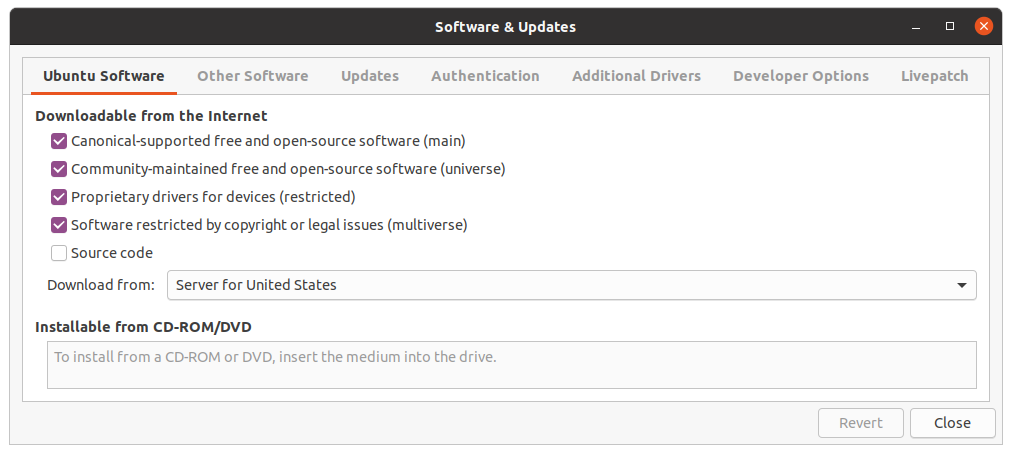
\includegraphics[scale=0.4]{cap02/progsAtualizacoes.png}
 \caption{Programas e Atualizações}
\end{figure}

Nesta primeira aba, mostrada na figura, define quais serão os aplicativos que estarão disponíveis na Loja. As opções são: \vspace{-1em}
\begin{itemize}[noitemsep]
 \item Main – possuem o suporte oficial da Canonical e dificilmente darão qualquer problema com o sistema operacional.
 \item Universe – mantidos pela comunidade, porém, não são oficiais dos desenvolvedores Ubuntu. 
 \item Restricted – proprietários e em sua maioria drivers necessários. 
 \item Multiverse – proprietários e de código fechado. 
\end{itemize}

A última aba se refere ao serviço da Canonical chamado de Livepatch. Tem a função de aplicar correções críticas no sistema sem a necessidade de reiniciar. Essas podem envolver segurança ou partes da infraestrutura de suporte a pacotes. Porém para acessar esse serviço é necessário primeiro criar uma conta (gratuita) na \textbf{Ubuntu One}.

\subsection{Dash}\index{Falando com Ubuntu}
Antes de começarmos a explorar alguns desses aplicativos (e outros) vamos falar da área na qual estão localizados que é conhecida como Dash - Para acessá-la clique no quadrado de pontinhos que fica no inferior da barra lateral:
\begin{figure}[H]
 \centering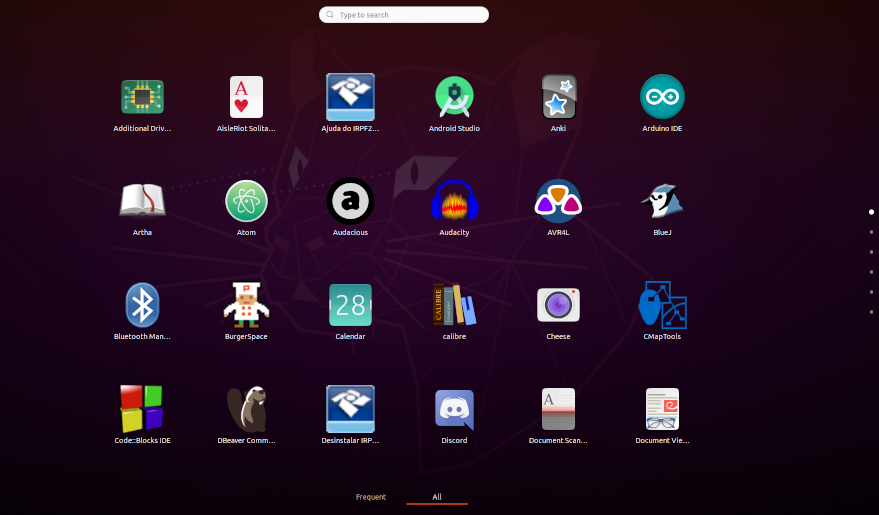
\includegraphics[scale=0.4]{cap02/dash.png}
 \caption{Dash}
\end{figure}

Poderia dizer que é a janela mais importante do sistema pois através desta é possível acessar todos os aplicativos disponíveis no sistema. Para acessar um determinado aplicativo basta digitar seu nome.
\\[3mm]
\begin{dica}[Usando aplicativos] A partir de agora toda vez que citar o aplicativo, bastará ir nessa janela e digitar seu nome, não farei mais referência a isso.
\end{dica}

Não tenha a menor vergonha de pedir ajuda, faço isso constantemente nesse sistema, abra o Dash e digite a palavra \textbf{ajuda} e a seguinte tela será mostrada:
\begin{figure}[H]
 \centering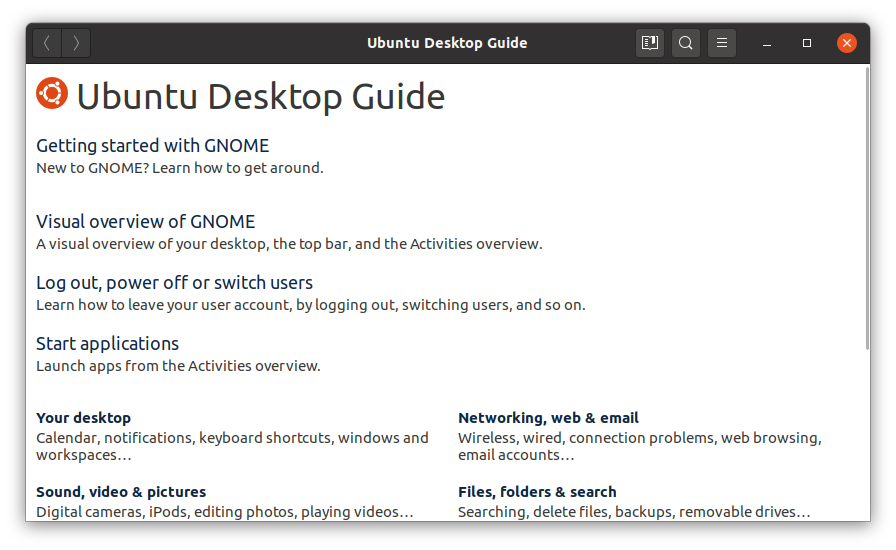
\includegraphics[scale=0.4]{cap02/ajuda.png}
 \caption{Janela de Ajuda}
\end{figure}

Explore muito bem essa janela como forma de fixar alguns conceitos ou para aprofundar ainda mais seu conhecimento sobre o sistema. Outro detalhe interessante do Dash é que também é possível acessar diretamente a loja para desinstalar um aplicativo. Realize uma pesquisa do aplicativo, clique com o botão direito do mouse sobre seu ícone e selecione a opção \textbf{Mostrar detalhes}.

\section{Loja de Aplicativos}\index{Falando com Ubuntu}
O aplicativo \textbf{Ubuntu Software} é a ``loja'' oficial da Canonical, normalmente seu ícone vem grudado na barra lateral como uma sacola alaranjada que nos leva ao painel principal do aplicativo e permite realizar buscas avançadas nos mais diversos aplicativos disponibilizados pelos repositórios.
\begin{figure}[H]
 \centering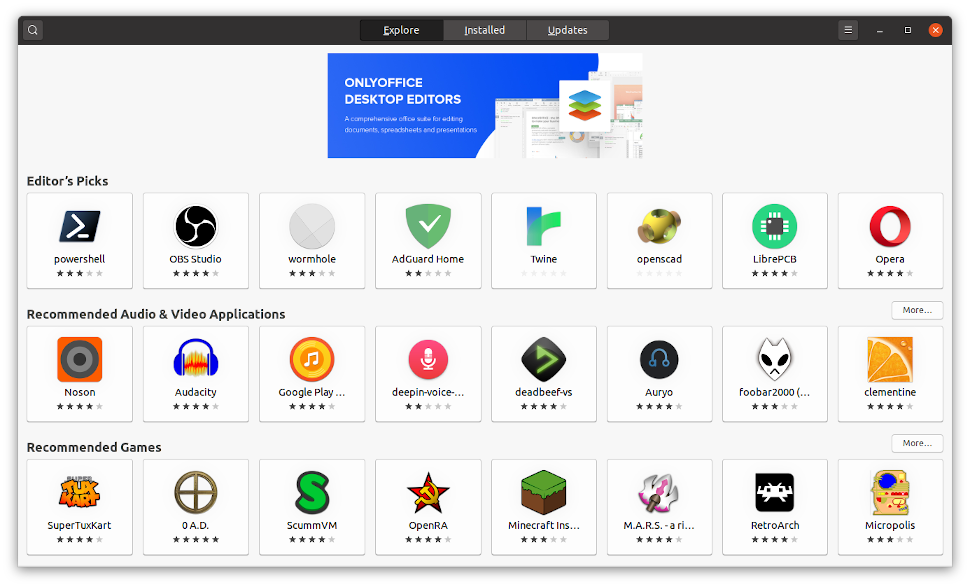
\includegraphics[scale=0.4]{cap02/loja.png}
 \caption{Ubuntu Software}
\end{figure}

Essa loja foi um dos melhores softwares criados nos últimos anos para Linux (e um grande avanço em relação a versões anteriores). Podemos dizer que foi a concretização do projeto original sobre os ``APT do Debian'' e buscava substituir por completo a instalação através da tela de terminal, além de ter uma espécie de ``supermercado de aplicativos'', no qual se escolhe, clica e instala. A instalação de um aplicativo é equivalente no terminal ao comando: \\
{\ttfamily\$ sudo apt install [nome-aplicativo]} 

No mundo dos derivados do Debian, existem os aplicativos com a extensão \textbf{.deb}\footnote{Para instalar este tipo de arquivo é necessário primeiramente instalar o \textbf{GDebi}, que pode ser localizado na loja} (que funcionam como se fossem os \textbf{.exe} do Windows) e esses arquivos permitem a instalação de softwares de terceiros sem ter que adicionar um repositório.
\\[3mm]
\begin{dica}[Sudo] Tenha sempre em mente que no mundo Linux existem dois usuários bem distintos, o seu usuário e o superusuário, e apenas para esse segundo que é permitido instalar ou remover aplicativos, então tenha sempre a mão a senha desse superusuário, que foi definida ao se instalar o sistema operacional.
\end{dica}
Para desinstalar quaisquer aplicativo no Ubuntu basta realizar essa ação através da Loja, ou conhecendo o nome correto do programa, digitar o seguinte comando no terminal: \\
{\ttfamily\$ sudo apt remove [nome-aplicativo]}

Como alternativa\footnote{Prefiro mais pensar na palavra: \textbf{complemento}} a loja, os usuários gostam de instalar o \textbf{Synaptic} que é um gerenciador de repositórios. Use-o com maior cuidado e atenção, pois assim que entramos nesse aplicativo a senha do superusuário deve ser informada, então o aplicativo possui o poder de realizar qualquer ação no seu sistema, inclusive a de remover pacotes que podem danificá-lo.

\section{Adicionar e Remover Repositórios}\index{Falando com Ubuntu}
Onde estão os aplicativos instalados através da loja? Se encontram na Internet em um endereço que para o sistema é conhecido como \textbf{Repositório}. Alguns repositórios são colocados por padrão no seu sistema, enquanto que outros devem ser adicionados.

Para adicionar um repositório os usuários comumente utilizam o terminal (inclusive em muitos sites é muito comum encontrar essa sintaxe), composta por dois comandos: \\
{\ttfamily\$ sudo add-apt-repository ppa:[Nome\_PPA]/ppa}

Venho frisando, desde o início deste livro, que possuo o desejo de tornar as coisas mais fáceis, então em vez de abrir um terminal para realizar este processo, acesse o \textbf{PA} e na aba \textbf{Outros Programas} e teremos a seguinte visão:
\begin{figure}[H]
 \centering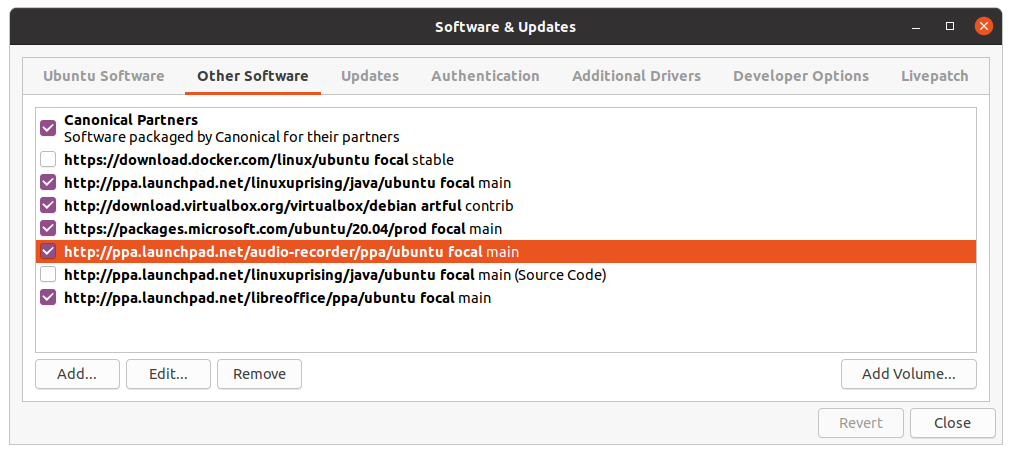
\includegraphics[scale=0.4]{cap02/outrosProgramas.png}
 \caption{Programas e atualizações, aba Outros Programas}
\end{figure}

Pessoalmente acho que essa aba deveria se chamar Repositórios, pois aí se localiza todos os repositórios disponibilizados pelo sistema. Ou seja, basta pressionar o botão \textbf{Adicionar...} e informar o local aonde está o repositório, com a seguinte sintaxe: \\
{\ttfamily deb http://ppa.launchpad.net/[Nome\_PPA]/ubuntu [codinome] main}

Por exemplo, um repositório que está na versão \textbf{Ubuntu 14.10} seria assim adicionado: \\
{\ttfamily deb http://ppa.launchpad.net/[Nome\_PPA]/ubuntu utopic main}

Note que apenas o substantivo do codinome da versão é usado. Ao fechar o aplicativo o equivalente ao comando do terminal é executado: \\
{\ttfamily\$ sudo apt update}

Para eliminar um repositório, basta localizá-lo e clicar no botão Remover. Isso corresponde ao seguinte comando do terminal: \\
{\ttfamily\$ sudo add-apt-repository ---remove ppa:[Nome\_PPA]}

Essa lista de repositórios, que visualizamos no aplicativo, também pode ser vista no terminal com o seguinte comando: \\
{\ttfamily\$ sudo ls /etc/apt/sources.list.d}

Com o repositório instalado basta ir na Loja e pesquisar pelo nome do aplicativo e instalá-lo sem maiores dificuldades, então quando, neste livro, houver a necessidade de instalar um repositório para um aplicativo apenas indicarei qual a composição do nome do repositório a instalar: \vspace{-1em}
\begin{itemize}[noitemsep]
 \item Repositório: [Nome\_PPA]
 \item Aplicativo: [Nome\_Aplicativo]
\end{itemize}

\subsection{E se um repositório não for reconhecido?}\index{Falando com Ubuntu}
Duas coisas podem ter acontecido, primeira o nome do repositório foi digitado incorretamente (verifique se o nome é realmente este) ou este repositório é incompatível com a versão do Ubuntu utilizada, neste caso não é recomendável a instalação do aplicativo (que pode ser forçada através dos comandos do terminal por sua conta e risco). Exatamente por este motivo que recomendo ao usuário leigo o uso da parte gráfica como forma de controlar melhor seus repositórios.

No caso de alguns softwares pode ocorrer que não apareça na loja pois esta não trabalha com qualquer repositório (que pode ser um de terceiro), então obrigatoriamente devemos instalá-lo a partir do terminal com o comando: \\
{\ttfamily\$ sudo apt install [nome]}

\subsection{Snappy – Um novo modelo de aplicativos}\index{Falando com Ubuntu}
O Ubuntu 16.10 trouxe o início de uma profunda mudança que é a disponibilização de um novo modelo de pacotes denominados Snappy (ou Snap\footnote{Snap pode ser traduzido para romper ou arrebentar, mas o sentido mais comum e estalo ou ruptura} como estão sendo apelidados). A grande vantagem deste novo modelo é a palavra ``Convergência'', no qual um mesmo pacote pode ser instalado em vários hardwares que contenham a versão do sistema operacional (desktop, tablets, celulares, e por aí vai). Seu uso ainda é modesto e centralizado (assim como no início dos pacotes APT) no terminal ou através da Internet no seguinte endereço \url{https://snapcraft.io/store}.

Encontrar os pacotes disponíveis: \\
{\ttfamily\$ snap find [aplicativo]}

Obter informações de algum pacote: \\
{\ttfamily\$ snap info [aplicativo]}

Instalar algum pacote: \\
{\ttfamily\$ sudo snap install [aplicativo]}

Verificar os pacotes que estão instalados no sistema: \\
{\ttfamily\$ snap list}

Obter um histórico das mudanças dos pacotes no sistema: \\
{\ttfamily\$ snap changes}

Realizar um upgrade para a nova versão: \\
{\ttfamily\$ sudo snap refresh [aplicativo]}

Remover um pacote: \\
{\ttfamily\$ sudo snap remove [aplicativo]}

Se é desenvolvedor, caso possua e deseja logar na conta do Ubuntu One: \\
{\ttfamily\$ sudo snap login [email]}

A Canonical está pressionando para torná-los um novo padrão ao Ubuntu e assim poder disponibilizar a Convergência. Foi lançada uma ferramenta chamada de \textbf{Snapcraft} de modo que será mais fácil os desenvolvedores criarem novos aplicativos em várias linguagens de programação. Acesse o site para descobrir vários pacotes que está a disposição neste novo formato: \url{https://uappexplorer.com/apps?type=snappy}

\subsection{Resumindo tudo e AppImage}\index{Falando com Ubuntu}
Então o que sabemos sobre os aplicativos do Ubuntu é que eles podem ser de três tipos: \vspace{-1em}
\begin{enumerate}[noitemsep]
 \item Pacote \textbf{deb}, que contém o aplicativo completo sem a necessidade de instalar um repositório.
 \item Pacote \textbf{snappy}, que também contém o aplicativo completo sem a necessidade de instalar um repositório.
 \item Aplicativo comum que pode ou não ter a necessidade de instalar um repositório extra.
\end{enumerate}

E como se nada disso fosse suficiente uma quarta forma está surgindo é chamada de \textbf{AppImage}, nesse formato não é necessário instalar absolutamente nada no seu sistema basta apenas baixar o arquivo, transformá-lo em um executável e clicar nele. Vamos tentar entender como isso funciona com um excelente software editor de partituras, acesse o site oficial em \url{https://musescore.org/pt-br/download}, localize e baixe a AppImage.

Abra o Nautilus (Gerenciador de Arquivos), localize a pasta /Downloads e clique com o botão direito do mouse sobre o arquivo baixado e acesse a aba \textbf{Permissões}. Marque a opção ``Permitir a execução do arquivo como um programa'', saia da tela e simplesmente clique no arquivo que o programa \textbf{MuseScore} será aberto sem ser realizada nenhuma instalação no seu sistema. 
\begin{figure}[H]
 \centering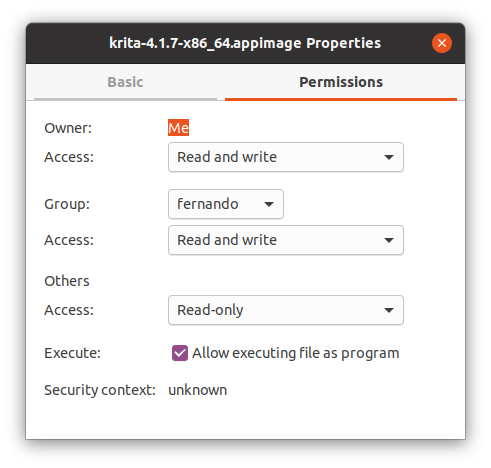
\includegraphics[scale=0.4]{cap02/executavel.png}
 \caption{Propriedades, aba Permissões}
\end{figure}

Calma que o mundo não é assim tão maravilhoso, a vantagem bem clara que é possível criar uma pasta e colocar diversos aplicativos nela sem ter que instalar (e sujar) absolutamente nada no seu sistema. Porém a desvantagem seria mais relacionada a atualização do aplicativo como não existe um repositório e esse arquivo está ``estável'' em seu sistema e não existirá a atualização do mesmo. Então minha recomendação é: \textit{use este tipo de pacote para testar um aplicativo, gostou e vai realmente usá-lo? Instale-o}.

\section{Atalhos ou Lançadores}\index{Falando com Ubuntu}
Uma das grandes diferenças entre os sistemas Windows e Linux é em relação aos Lançadores (\textbf{Atalhos} é coisa de Windows). No Windows são arquivos misteriosos que pouca gente sabe seu conteúdo, sabe simplesmente que se clica com o botão direito sobre um executável (aqui não existe esse conceito) e seleciona a opção ``Criar atalho'' então a mágica acontece. 

No Linux são arquivos com a extensão \textbf{.desktop} e que possuem a permissão de serem executados pelo sistema (uma vez que estão corretamente definidos). Residem na pasta /usr/share/applications (o Dash só reconhece as aplicações que estão nesta pasta), mas para um usuário que vem do Windows a primeira tendência é a de copiar um punhado deles para a \textbf{Área de Trabalho}.

Esses arquivos possuem uma estrutura definida, vejamos como exemplo o lançador que chama o aplicativo que controla o \textbf{Brilho \& Bloqueio}:
\begin{lstlisting}
[Desktop Entry]
Name=Brightness & Lock
Comment=Screen brightness and lock settings
Exec=unity-control-center screen
Icon=system-lock-screen
Terminal=false
Type=Application
Categories=GNOME;GTK;Settings;DesktopSettings;X-Unity-Settings-Panel
\end{lstlisting}

Observamos que é quase um arquivo auto explicativo (retirei algumas variáveis desnecessárias a fim de visualizarmos melhor o arquivo) e a única coisa que devemos ter em mente é que a variável \textbf{Exec} chamará o aplicativo, sendo que o comando colocado aqui seria o seu equivalente a tela de terminal. E um lançador estará criado pois as outras variáveis são simples informações. Recomendo que use este arquivo como um modelo para criar seus próprios lançadores quando houver necessidade.

\subsection{Entre o Nano e o gEdit}\index{Falando com Ubuntu}
A briga entre o ambiente gráfico e não gráfico é muito estranha, vamos comparar esses dois editores. Várias vezes precisamos editar arquivos que não podem ganhar ``caracteres estranhos'' como os colocados por aplicativos como Writer (LibreOffice) ou MS-Word (MS-Office), assim precisamos utilizar de editores mais simples, no Windows seria o equivalente ao ``Bloco de Notas''.

Existem para o ambiente Linux dois excelentes editores: \textbf{Nano} e \textbf{gEdit}, a diferença? O primeiro não é gráfico e o segundo totalmente gráfico. Abra uma janela de terminal e digite o comando: \\
{\ttfamily\$ nano}

E a seguinte tela será chamada:
\begin{figure}[H]
 \centering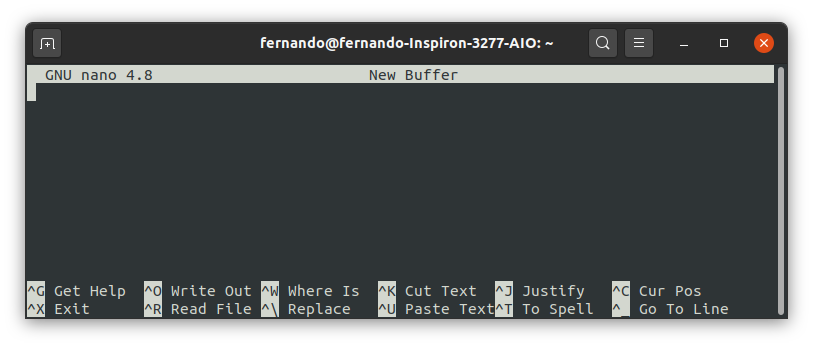
\includegraphics[scale=0.4]{cap02/nano.png}
 \caption{Editor Nano}
\end{figure}

Os comandos do editor estão expostos na barra do rodapé, sendo que o caractere circunflexo corresponde a tecla \textbf{Ctrl}, ou seja, para gravar pressionamos \textbf{Ctrl + O}, sair do editor \textbf{Ctrl + X} e assim sucessivamente. Outro detalhe interessante é possível pará-lo, retornar ao terminal, proceder alguma ação e retornar ao editor. Isso é chamado de Job (trabalho). Guarde bem os seguintes comandos: \vspace{-1em}
\begin{itemize}[noitemsep]
 \item No nano pressione \textbf{Ctrl + Z} para parar o job.
 \item No terminal escreva: {\ttfamily jobs}, para ver os jobs que estão parados. 
 \item No terminal escreva: {\ttfamily fg [n]}, para retornar a um job parado. 
\end{itemize}

Já o gEdit, por ser um programa gráfico, pode ser acessado de três maneiras diferentes: \vspace{-1em}
\begin{enumerate}[noitemsep]
 \item Abrir o aplicativo ``Editor de Textos'' no Dash
 \item Pressionar \textbf{Alt + F2} e digitar {\ttfamily gedit}
 \item Através do seguinte comando no terminal: {\ttfamily\$ gedit}.
\end{enumerate}

O efeito será o mesmo e a seguinte tela será mostrada:
\begin{figure}[H]
 \centering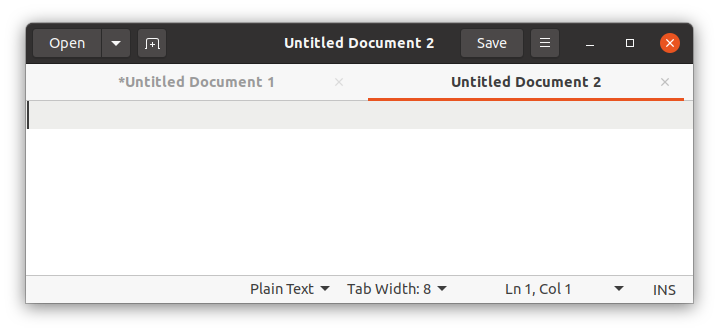
\includegraphics[scale=0.4]{cap02/gedit.png}
 \caption{Editor gEdit}
\end{figure}

Ou seja, trabalhar com um ou outro torna-se apenas uma questão de gosto pessoal. Porém, pode existir o caso do ambiente gráfico não estar presente e assim o Nano acaba por tornar a única ponte de salvação para a edição dos arquivos, a menos que prefira algo como \textbf{Vi} que já disse se tratar da obra do Demônio.

\subsection{Entre o chmod e o Nautilus}\index{Falando com Ubuntu}
Meio estranho dizer isso no título pois um deles é apenas um simples comando para modificar as permissões de um arquivo enquanto que o outro é um gerenciador de arquivos. No Nautilus basta clicar com o botão direito sobre qualquer arquivo e acessar a aba \textbf{permissões}. 

Ou então entrar no terminal e digitar (em qualquer pasta que existam arquivos) o seguinte comando: \\
{\ttfamily\$ ls -l}

Na listagem dos arquivos (logo na primeira coluna) aparecerá algumas letras, entre elas: d, r, w e x. Estas letras são permissões e se divide nos seguintes grupos: Dono (ou proprietário), Grupo e Outros. As letras podem ser: \vspace{-1em}
\begin{itemize}[noitemsep]
 \item r – listar o conteúdo de pastas ou ler arquivos
 \item w – gravar em arquivos ou  pastas
 \item x – recursivo na árvore de pastas
 \item X – execução
 \item s – novos arquivos ou diretórios
 \item d – indicação de pasta
 \item Não aparecer a letra – herança da pasta
\end{itemize}

Porém o comando \textbf{chmod} também permite que façamos as trocas dessas permissões através do terminal, sua formação é realizada pelas letras ou por valores. Esse são os seguintes: \vspace{-1em}
\begin{itemize}[noitemsep]
 \item 0 – nada
 \item 1 – execução
 \item 2 – gravação
 \item 4 – leitura
\end{itemize} 

O somatório dos números também é válido, ou seja, para dar permissão de leitura e gravação usamos o número 6, já leitura e execução o 5 e assim sucessivamente. Por exemplo para dar permissão completa a um arquivo, podemos digitar o seguinte comando: \\
{\ttfamily\$ chmod 0777 nomearquivo}

O que é esse primeiro número? A informação deve ser passada em base Octal, e essa começa por 0. Para usarmos as letras, o sinal de soma (+) adiciona uma permissão, enquanto que o sinal de subtração (-) remove a permissão, então o mesmo comando poderia ser descrito da seguinte forma: \\
{\ttfamily\$ chmod a+rwx nomearquivo}

O significado é que o primeiro ``a'' é uma notação que indica modo de adição dos valores, podemos também usar ``i'' que indica imutabilidade ou ``s'' indicando segurança para exclusão. Quando usar um ou outro? Tanto faz, normalmente o que ficar mais simples. Por exemplo, para dar permissão de leitura e gravação para o usuário, apenas leitura para o grupo e outros. Para utilizar números resolvemos assim: \\
{\ttfamily\$ chmod 0644 nomearquivo}

Já com letras deveriamos realizar vários comandos para conseguirmos isso. Já para dar permissão de execução (por exemplo a um Script), bastaria digitar: \\
{\ttfamily\$ chmod +x nomearquivo}

Permissões em arquivos ou pastas são muito importantes, recomendo que aprenda as duas formas de trabalhar pois, como disse, nunca se sabe quando o terminal se tornar a única opção.

% Final do Capítulo
\clearpage